\label{chap.5}
\label{chap:mabms_architecture}

\section{System Architecture and Information Flow}
\label{sec:ch5_architecture}

The MA-BMS partitions fast-charging control into modular functional entities where proposer agents generate advisory recommendations and an analytical supervisor deterministically validates commands before plant actuation (Figure~\ref{fig:mabms_arch}).
\begin{figure}[htbp]
    \centering
    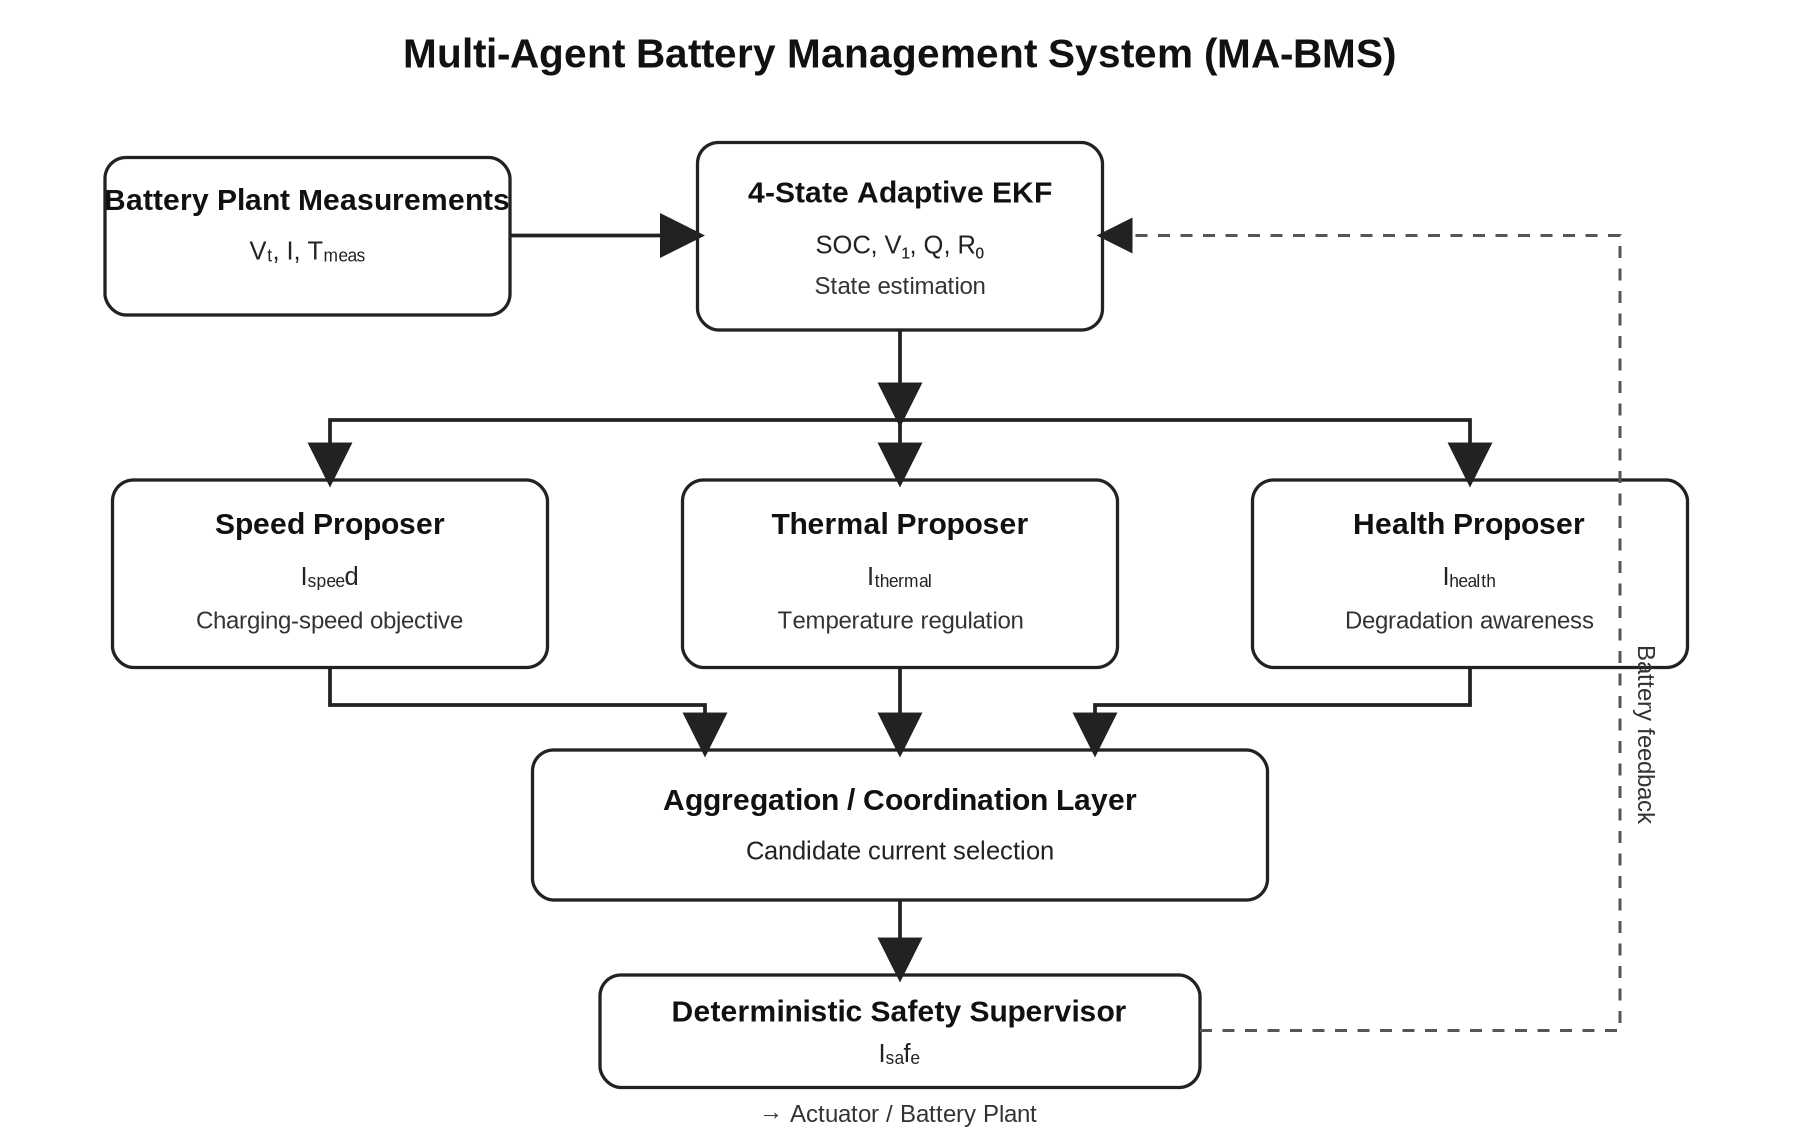
\includegraphics[width=0.95\textwidth]{MA_BMS_Architecture.png}
    \caption{MA-BMS modular architecture and information flow.}
    \label{fig:mabms_arch}
\end{figure}
The execution sequence at each discrete time step $k$ proceeds as:
\begin{enumerate}
    \item Sample telemetry: pack terminal voltage $V_t$, current $I$, and surface temperature $T_{\mathrm{meas}}$.
    \item Execute the adaptive EKF time and measurement updates to obtain state estimate $\hat{\mathbf{x}}_k = [\widehat{\mathrm{SOC}}_k, \hat{V}_{1,k}, \hat{b}_k, \hat{\rho}_k]^\top$.
    \item Broadcast $\hat{\mathbf{x}}_k$, thermal limits, and deadline parameters to the proposer agents.
    \item Collect candidate actions from each agent and synthesise a candidate current command at the coordination layer.
    \item Enforce analytical voltage bounds and thermal plausibility checks via the deterministic supervisor.
    \item Apply the certified current to the cell hardware or simulated battery plant.
\end{enumerate}

\section{Proposer Agents and Their Responsibilities}
\label{sec:ch5_agents}

Each proposer agent optimises a dedicated operational dimension without direct actuator authority.

\subsection{Charging-Speed Proposer}
\label{subsec:ch5_speed_agent}

The charging-speed proposer prioritises rapid target SOC attainment. Based on estimated state $\widehat{\mathrm{SOC}}_k$, target $\mathrm{SOC}^{*}$, and time remaining to deadline $t_{\mathrm{rem}}$, it computes nominal charging current $I_{\mathrm{speed}}$. The proposal is aggressive during early charging phases and tapers as the target SOC is approached. It remains unconstrained by internal stress models, delegating boundary enforcement downstream.

\subsection{Thermal-Regulation Proposer}
\label{subsec:ch5_thermal_agent}

The thermal-regulation proposer limits cell temperature rise. Given temperature $T_k$, ambient $T_{\mathrm{amb}}$, and maximum allowable limit $T_{\mathrm{crit}}$, it computes:
\begin{equation}
  I_{\mathrm{thermal}} = \sqrt{\frac{h (T_{\mathrm{crit}} - T_{\mathrm{amb}})}{\hat{\rho}_k R_0}},
\end{equation}
representing the steady-state thermal current headroom. By throttling current as $T_k \to T_{\mathrm{crit}}$, it prevents thermal runaway risk while maintaining active charging throughput.

\subsection{Health/Degradation Proposer}
\label{subsec:ch5_health_agent}

The health/degradation proposer bounds high-current and high-SOC exposure. To mitigate accelerated capacity fade and mechanical stress, it recommends a health-oriented current cap:
\begin{equation}
  I_{\mathrm{health}} = k_{\mathrm{cap}} \cdot C_{\mathrm{nominal}},
  \label{eq:health_cap}
\end{equation}
where $k_{\mathrm{cap}} \in (0, 1]$ modulates peak current scaling (e.g., $k_{\mathrm{cap}} = 0.70$ for the health-cap benchmark).

\section{Coordination and Proposal Aggregation}
\label{sec:ch5_coordinator}

The coordination layer arbitrates between conflicting agent proposals. While the speed proposer requests maximal permissible current to satisfy deadlines, the thermal and health proposers advocate conservative bounds. The primary baseline aggregation policy applies a conservative bound:
\begin{equation}
  I_{\mathrm{cand}} = \min\bigl(I_{\mathrm{speed}},\, I_{\mathrm{thermal}},\, I_{\mathrm{health}}\bigr).
\end{equation}
In multi-objective optimization settings, weighted consensus $I_{\mathrm{cand}} = \sum_j w_j I_j$ is evaluated. In all cases, candidate command $I_{\mathrm{cand}}$ is passed to the safety supervisor for deterministic verification prior to application.

\section{Four-State Adaptive Extended Kalman Filter}
\label{sec:ch5_estimator}

\subsection{State Vector and System Dynamics}
\label{subsec:ch5_state_dynamics}

Accurate battery management requires real-time tracking of unmeasurable electrochemical states under ageing. The four-state adaptive EKF models state of charge ($\mathrm{SOC}$), RC polarisation voltage ($V_1$), capacity degradation factor ($b = Q_{\mathrm{nom}} / Q_{\mathrm{actual}}$), and ohmic resistance scale factor ($\rho = R_{0,\mathrm{actual}} / R_{0,\mathrm{nominal}}$).

The augmented state vector is defined as:
\begin{equation}
  \mathbf{x}_k = \begin{bmatrix} \mathrm{SOC}_k & V_{1,k} & b_k & \rho_k \end{bmatrix}^\top.
\end{equation}
The discrete-time state transition equations are:
\begin{align}
  \mathrm{SOC}_{k+1} &= \mathrm{SOC}_k - \frac{I_k \Delta t}{Q_{\mathrm{nom}} / b_k}, \\
  V_{1,k+1} &= V_{1,k} e^{-\Delta t/\tau_1} + I_k R_1 \left(1 - e^{-\Delta t/\tau_1}\right), \\
  b_{k+1} &= b_k + w_{b,k}, \qquad w_{b,k} \sim \mathcal{N}(0, \sigma_b^2), \\
  \rho_{k+1} &= \rho_k + w_{\rho,k}, \qquad w_{\rho,k} \sim \mathcal{N}(0, \sigma_\rho^2),
\end{align}
where $\Delta t$ is the sampling interval, $\tau_1 = R_1 C_1$ is the diffusion time constant, and $w_{b,k}, w_{\rho,k}$ represent Gaussian random-walk process noise.

The nonlinear observation equation for pack terminal voltage is:
\begin{equation}
  V_k = V_{\mathrm{OCV}}(\mathrm{SOC}_k) - I_k \rho_k R_0 - V_{1,k} + \nu_k, \quad \nu_k \sim \mathcal{N}(0, \sigma_V^2),
\end{equation}
with measurement Jacobian:
\begin{equation}
  \mathbf{H}_k = \left. \frac{\partial V_k}{\partial \mathbf{x}} \right|_{\hat{\mathbf{x}}_k^-} = \begin{bmatrix} \left.\frac{d V_{\mathrm{OCV}}}{d\mathrm{SOC}}\right|_{\widehat{\mathrm{SOC}}_k^-} & -1 & 0 & -I_k R_0 \end{bmatrix}.
\end{equation}

\subsection{Ageing-Aware Parameter Initialisation}
\label{subsec:ch5_ageing_init}

To minimise transient estimator error at start-of-test on aged cells, the initial resistance scale factor is seeded from the estimated initial State of Health ($\widehat{\mathrm{SOH}}_0$):
\begin{equation}
  \rho_0 = f_{R_0}(\widehat{\mathrm{SOH}}_0) = 1 + k_{R_0}^{\mathrm{est}} \cdot \left(1 - \widehat{\mathrm{SOH}}_0\right),
\end{equation}
with $k_{R_0}^{\mathrm{est}} = 3.0$ derived from the empirical regression established in Chapter~3. This eliminates early voltage mismatch before EKF convergence.

\section{Deterministic Safety Supervisor}
\label{sec:ch5_safety}

The deterministic safety supervisor serves as the uncompromised final authority. It enforces explicit electro-thermal constraints upstream of the actuator.

\subsection{Analytical Voltage Bounds}
\label{subsec:ch5_voltage_bounds}

To prevent overvoltage during aggressive charging, the supervisor computes an analytical maximum safe current bound $I_{\mathrm{safe}}$ at each step:
\begin{equation}
  I_{\mathrm{safe}} = \frac{V_{\mathrm{max}} - \hat{V}_{\mathrm{OCV}} - \Delta V_{\mathrm{margin}}}{\hat{\rho} \, R_0 + R_{\mathrm{cable}}},
  \label{eq:i_safe}
\end{equation}
where $V_{\mathrm{max}} = \SI{8.4}{V}$ is the pack limit, $\hat{V}_{\mathrm{OCV}} = V_{\mathrm{OCV}}(\widehat{\mathrm{SOC}})$, and $R_{\mathrm{cable}}$ accounts for interconnect parasitics. The dynamic safety margin is formulated as:
\begin{equation}
  \Delta V_{\mathrm{margin}} = I_{\mathrm{nominal}} \cdot R_0 \cdot (\gamma_{R_0} - 1),
\end{equation}
with $\gamma_{R_0} = 1.30$. The candidate command is strictly clamped:
\begin{equation}
  I_{\mathrm{exec}} = \max\Bigl(0,\, \min\bigl(I_{\mathrm{cand}},\, I_{\mathrm{safe}},\, I_{\mathrm{max}}\bigr)\Bigr).
\end{equation}

\subsection{Thermal Plausibility Monitoring}
\label{subsec:ch5_thermal_monitor}

Thermal safety is augmented by real-time residual plausibility checks between measured cell temperature $T_{\mathrm{meas}}(t)$ and the lumped thermal model prediction $\hat{T}(t)$:
\begin{equation}
  r_T(t) = T_{\mathrm{meas}}(t) - \hat{T}(t).
\end{equation}
If $|r_T(t)| > \Delta T_{\mathrm{thresh}} = \SI{4.0}{\degreeCelsius}$ persists for $k \ge 5$ consecutive steps, a sensor fault is triggered. The supervisor overrides active control to a safe fallback rate $I_{\mathrm{exec}} = \SI{0.5}{A}$.

\subsection{Safety Boundary and Reporting}
\label{subsec:ch5_safety_boundary}

The supervisor guarantees hard physical bounds within the validity domain of the underlying ECM and thermal model. The experimental evaluation in Section~\ref{sec:ch5_evaluation} further assesses constraint adherence under sensor-fault conditions.

\section{Benchmark Controller Definitions}
\label{sec:ch5_baselines}

To evaluate the proposed architecture, four benchmark controller implementations are defined.

\subsection{Single-Agent Tuned Policy}
\label{subsec:ch5_single_agent}

A parameterised centralised policy that simultaneously regulates charging current and thermal cooling. The control parameters (base C-rate, proportional thermal gain, temperature setpoint, and deadline gain) are optimised via offline random search over a composite multi-objective scalar reward $J$.

\subsection{Independent-Deadline Baseline}
\label{subsec:ch5_independent_baseline}

An analytical controller targeting constant current profiles calculated to meet the charging deadline:
\begin{equation}
  I_{\mathrm{indep}} = \frac{Q_{\mathrm{nom}} (\mathrm{SOC}^{*} - \widehat{\mathrm{SOC}})}{t_{\mathrm{rem}}},
\end{equation}
subject to clamping by the deterministic safety supervisor.

\subsection{Health-Cap Controller}
\label{subsec:ch5_health_baseline}

An extension of the Independent-Deadline controller enforcing the degradation current cap defined in Eq.~\ref{eq:health_cap} ($k_{\mathrm{cap}} = 0.70$, capping current to \SI{1.75}{A}). It explicitly evaluates the trade-off between battery stress mitigation and deadline adherence.

\subsection{Conventional CC-CV Baseline}
\label{subsec:ch5_cccv}

The industry-standard CC-CV reference. Applies constant current $I_{\mathrm{cc}} = \SI{3.0}{A}$ until the upper voltage limit $V_{\mathrm{max}} = \SI{8.4}{V}$ is reached, followed by constant voltage regulation until current tapers to $I_{\mathrm{cutoff}} = \SI{0.3}{A}$.

\section[Experimental Evaluation of the Framework]{Experimental Evaluation of the Proposed Framework}
\label{sec:ch5_evaluation}

The proposed architecture is evaluated using unseen test episodes to assess charging completion, estimation accuracy, execution time, and safety adherence. The evaluation compares the four controller configurations defined in Section~\ref{sec:ch5_baselines} and isolates the contribution of the adaptive EKF through an ablation study.

\subsection{Experimental Setup}

The evaluation uses the same battery model, charging target, operating constraints, estimator configuration, and controller settings described in the preceding sections. Each controller is tested under the same unseen test conditions so that differences in performance can be attributed to controller and estimator configuration rather than changes in the evaluation protocol.

\subsection{Evaluation Metrics}

Performance is quantified using deadline success rate, SOC shortfall, SOC mean absolute error (MAE), charging time, and unsafe control steps per episode. These metrics jointly measure the ability to meet the charging objective, estimate battery state accurately, complete charging efficiently, and remain within the imposed safety boundary.

\subsection{Controller Evaluation Protocol}

The four configurations are evaluated using the Single-Agent, Independent-Deadline, Health-Cap, and Conventional controller definitions. For each configuration, the adaptive four-state EKF is compared with a two-state fixed-parameter EKF while keeping the remaining controller conditions unchanged.

\subsection{Overall Controller Performance}

The experimental results compare the controller configurations using the metrics defined above. The comparison is intended to identify the trade-off between charging speed, deadline attainment, state-estimation accuracy, and conservative health or safety constraints.

\subsection{Safety and Constraint Evaluation}

Safety performance is assessed from the number of unsafe control steps and the operation of the deterministic supervisor. The supervisor remains the final authority over all candidate commands; therefore, proposer recommendations cannot directly bypass the analytical voltage and thermal checks.

\subsection{Comparative Analysis of Controller Configurations}

The controller results are interpreted jointly rather than through a single objective. Faster controllers may reduce charging time but require greater reliance on accurate state estimation and safety enforcement, whereas health-oriented controllers may sacrifice completion speed to reduce battery stress. This comparison provides the basis for evaluating the proposed modular coordination strategy.

\subsection{EKF Ablation Analysis}

To quantify the contribution of joint capacity and resistance tracking, an ablation experiment evaluated the four-state adaptive EKF against a standard two-state fixed-parameter EKF ($\mathbf{x}=[\mathrm{SOC},V_1]^\top$) across four controller configurations over unseen test episodes (Table~\ref{tab:ekf_ablation}).

\begin{table}[htbp]
  \centering
  \caption{Ablation comparison of the 4-state adaptive EKF vs.\ 2-state fixed EKF across controllers.}
  \label{tab:ekf_ablation}
  \resizebox{\columnwidth}{!}{%
  \begin{tabular}{llccccc}
    \toprule
    \textbf{Controller Variant} & \textbf{EKF Scheme} & \textbf{Success Rate} & \textbf{SOC Shortfall} & \textbf{SOC MAE} & \textbf{Time (\si{s})} & \textbf{Unsafe Steps/Ep.} \\
    \midrule
    Conventional & Adaptive & 0.878 & 0.0048 & 0.0188 & 2391 & 0.178 \\
    Conventional & Fixed    & 0.700 & 0.0071 & 0.0228 & 2483 & 0.167 \\
    \addlinespace
    Independent  & Adaptive & 0.933 & 0.0038 & 0.0189 & 2371 & 0.144 \\
    Independent  & Fixed    & 0.722 & 0.0063 & 0.0228 & 2471 & 0.133 \\
    \addlinespace
    Health Cap   & Adaptive & 0.700 & 0.0136 & 0.0112 & 3952 & 0.000 \\
    Health Cap   & Fixed    & 0.633 & 0.0157 & 0.0164 & 3868 & 0.000 \\
    \addlinespace
    Single Agent & Adaptive & \textbf{1.000} & \textbf{0.0034} & 0.0338 & \textbf{1398} & \textbf{0.000} \\
    Single Agent & Fixed    & 0.900 & 0.0043 & 0.0339 & 1777 & 0.122 \\
    \bottomrule
  \end{tabular}%
  }
\end{table}

The adaptive EKF improves deadline success for all four controller configurations: by 17.8 percentage points for Conventional, 21.1 percentage points for Independent, 6.7 percentage points for Health Cap, and 10.0 percentage points for Single Agent, which reaches 100\% success. SOC shortfall is also reduced by approximately 20--32\% across the configurations. For the Single-Agent policy, unsafe steps decrease from 0.122 to 0.000 per episode, indicating improved safety-boundary adherence when adaptive estimation is used.

\subsection{Discussion of Experimental Findings}

Overall, the results indicate that the modular architecture separates objective-specific decision making from deterministic safety enforcement while allowing the estimator to adapt to battery ageing. The ablation results are consistent with a useful contribution from joint capacity and resistance tracking, particularly for deadline attainment and safety adherence. These findings support the use of adaptive state estimation as an integral component of the proposed MA-BMS rather than as an isolated monitoring module.

\section{Chapter Summary}
\label{sec:ch5_summary}

This chapter presented and evaluated the proposed modular MA-BMS framework. The architecture combines three objective-specific proposer agents for charging speed, thermal regulation, and degradation management; a coordination layer for candidate-current selection; a four-state adaptive EKF for online tracking of SOC, polarisation, capacity fade, and resistance growth; and a deterministic safety supervisor for analytical voltage and thermal protection. Four benchmark controllers were defined to provide consistent comparison, and experimental evaluation showed the contribution of adaptive estimation across controller configurations. The chapter therefore establishes both the control architecture and the experimental basis used to assess its effectiveness.